\documentclass{letter}
\usepackage{wallpaper}
\usepackage{geometry}
\usepackage{xcolor}
\usepackage[T1]{fontenc}
\usepackage[scaled]{helvet}
\usepackage{fontawesome5}
\usepackage{hyperref}
\usepackage[none]{hyphenat}
\usepackage{enumitem}
\usepackage{graphicx}
\usepackage{multicol}
\graphicspath{ {./img/} }

\setitemize{noitemsep, topsep=0.05em, leftmargin=0.2in, itemsep=0.05em}
\setlength{\columnsep}{5cm}

\renewcommand{\familydefault}{\sfdefault}

\geometry{
  paperwidth=\dimexpr\textwidth+\marginparsep+\marginparwidth\relax,
  paperheight=\dimexpr\textheight+\footskip\relax,
  left=20pt,
  right=20pt,
  top=0pt,
  bottom=0pt,
  nohead,
  nofoot,
  nomarginpar
}

\ThisCenterWallPaper{1.5}{cvbg.png}

\begin{document}

\begin{minipage}[t]{0.40\textwidth}
\setlength{\baselineskip}{1.5\baselineskip}
\color{white}
\vspace{1cm}
{\large Información personal}

\rule{\linewidth}{0.4pt}

\faPhone \quad \input{phone.tex} 
% Check phoneExample.tex

\faEnvelope \quad \href{malfi.bruno@gmail.com}{malfi.bruno@gmail.com}


\faMapMarker \quad Valencia

\rule{\linewidth}{0.4pt}

{\large Links}

\faLinkedin \quad \href{https://www.linkedin.com/in/bruno-malfi-fabeiro}{Linkedin}

\faGithub \quad \href{https://github.com/BrunoMalfi}{Github}

\faPaperclip \quad \href{https://github.com/BrunoMalfi}{CV extendido}

\rule{\linewidth}{0.4pt}

{\large Lenguajes}

\faNode \quad Node.js

\faReact \quad React

\faVuejs \quad Vue

\faAngular \quad Angular

\faLinux \quad Bash

\faCircleNotch \quad XSLT


\rule{\linewidth}{0.4pt}

{\large Idiomas}

\faLanguage \quad Español

\faLanguage \quad Inglés

\faLanguage \quad Italiano

\end{minipage}
\hfill
\begin{minipage}[t]{0.60\textwidth}
\setlength{\baselineskip}{1.5\baselineskip}
\vspace{0.8cm}

\begin{minipage}{0.8\linewidth} 
    {\huge Bruno Malfi Fabeiro}

    {\large Programador}
\end{minipage}
\begin{minipage}{0.1\linewidth}
    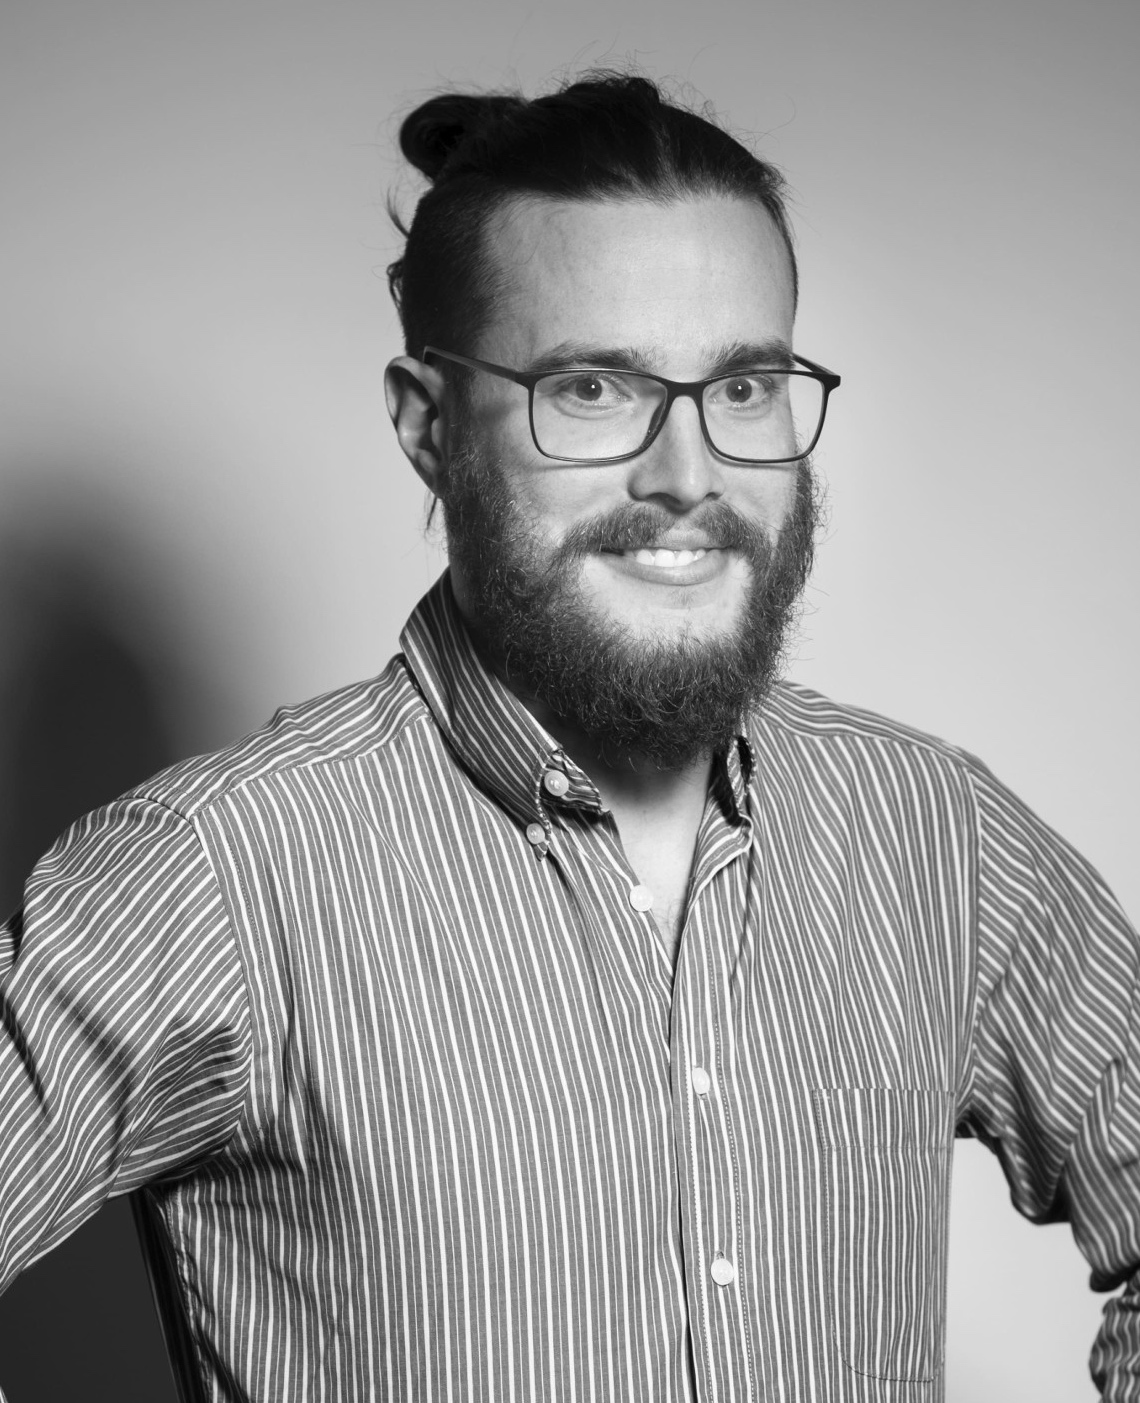
\includegraphics[width=1.5cm, height=2cm]{foto2.jpg}
\end{minipage}

\vspace{0.2cm}
 
9 años de experiencia en el sector IT. 
FP, Ingenieria y bootcamp FullStack.
Pero, sobre todo, con ganas de nuevos desafios

\vspace{0.5cm}

{\large Experiencia Laboral}
\rule{\linewidth}{0.4pt}
{\large \textbf{Programación FullStack}}

{\small MAR 2024 - Actualidad}

\begin{itemize}
    \item Proyectos en HTML, CSS y JavaScript Vanilla.
    \item  Backend en Node.js usando Express, Sequelize, Mongoose, etc.
    \item  Frontend, principalmente en React pero también en Vue y Angular.
\end{itemize}

{\large \textbf{Consultor/Técnico EDI, Freelance}}

{\small SEP 2018 - MAR 2024}

\begin{itemize}
    \item Consultoría EDI para clientes de DWID/Hillside.
    \item Consultoría EDI para clientes de ETRIS BANK.
    \item Mapas en XSLT. Scripts in Linux Bash.
\end{itemize}


{\large \textbf{Consultor/Técnico EDI en DERWID (Villach, Austria)}}

{\small JUL 2017 – SEP 2018}

\begin{itemize}
    \item Consultoría EDI para clientes de Derwid.
    \item Mapas en XSLT. Scripts in Linux Bash.
    \item Configuración de tablas mySQL con Workbench o PhpMyAdmin.
\end{itemize}

{\large \textbf{Consultor/Técnico EDI en EDICOM (Valencia)}}

{\small MAY 2015 - MAY 2017}
\begin{itemize}
    \item Mapas EbiMap. Scripts Javascript. 
\end{itemize}

{\large Education}
\rule{\linewidth}{0.4pt}

{\large \textbf{Bootcamp FullSatck Developer, EDEM (Master)}}

{\small MAR 2024- JUL 2024}

{\large \textbf{Ingeniería en Telecomunicaciones, UPV (Grado)}}

{\small SPT 2011- JUN 2015}


\end{minipage}
\end{document}